\Chapter{Saját Stratégiák}

Az AI felépítésénél a fókuszom egy olyan megvalósítás volt, ami egy egyszerű útvonalon lévő utasok szállításával foglalkozik a városok között, buszok használatával. Emiatt a lényegi része a programnak csak a közúti folyamatokkal foglalkozik. Másik szempontja volt a fejlesztésnek, hogy a program minél modulárisabb legyen, azaz a meglévő osztályok önállóan is tudjanak funkcionálni, és a kódban máshol is újra tudjuk őket hasznosítani, valamint az AI minél könnyebben kiegészíthető legyen egyéb funkcionalitásokkal.

\Section{Osztályok}

Az első feladat az különböző feladatok széttagolása. Ezt az alábbi különböző részekre osztottam:

\begin{itemize}
	\item Az AI játékmenetének a koordinálása
	\item Felállítandó vonalak keresése
	\item Városokon belüli tevékenységek kezelése
	\item Útépítéssel kapcsolatos funkciók
	\item Vonalak és azokhoz tartozó járművek kezelése
	\item Pénzügyek kezelése
\end{itemize}

Mindezeknek a feladatoknak az ellátása több kisebb szintű problémához vezet amiket az implementáció során külön-külön oldottam meg, ötletet merítve a kezdetleges próbálkozásokból és korábbi implementációkból.

Ahhoz hogy az AI a célját elérje és városok között utasokat tudjon szállítani buszok segítségével szüksége van az összes többi komponens megfelelő működésére. Az AI koordinálása értjük azt a pontot ahol ez megtörténik, és a többi alrész eredménye itt összegződik és valósul meg. Itt kell kezelnie a programnak az esetlegesen jelentkező problémákat is, ugyanis ha már elkezdett kiépíteni egy útvonalat, de annak befejezése nem valósult meg, akkor vagy vissza kell vonnia az addig befejezett elemeket, vagy pedig újrapróbálni a folyamatot.

Az egyik ilyen fontos komponens a vonalak létrehozásának szempontjából a tervező, amely segítségével le tudjuk kérdezni hogy hova lenne érdemes új buszvonalakat létrehozni az AI-nak.

Miután az ideális útvonalak városai rendelkezésre állnak, akkor szükség van egy olyan modulra, amely képes a városon belüli tevékenységeket kezelni. Gondolok ezalatt például a buszmegállók helyének meghatározására és megépítésére.

Ugyanakkor, ha a program által ismertek a városok amelyek között az ideális útvonalat létre kellene hoznunk, ahhoz hogy az utasokat el is tudjuk szállítani szükség lesz egy olyan modulra, amely képes a megfelelő városokat összekötni egy útvonallal költség és idő hatékony módon.

Az utasok szállításához végső sorban szükség van járművekre amelyek ezt a feladatot ellátják, így létrehoztam egy olyan modult is, amely az adott vonalhoz tartozó buszokat megvásárolja, irányítja, karban tartja és kezeli.

A korábban felsorolt tevékenységekhez természetesen a cégnek pénzre is szüksége van, így szükséges egy olyan modul amely biztosítja a cégnek azt az összeget amit igényel a feladatok ellátására, valamint a kölcsön összegét is kezeli.


\Section{Átfogó működés és irányítás}

A programkódunk main függvényében történik meg a hívás ami elindítja az AI folyamatot a játékon belül, ezért itt történnek meg a lényeges részei a programnak, mint például a cég létrehozása és a fő munkafolyamat leírása. Ennek a folyamatábrája \aref{fig:folyamat} ábrán látható. Mivel a játék célja egy infrastruktúra kiépítése és jövedelem generálása, így ezt a két dolgot itt kell körvonalaznom. Ez az osztály szolgál az AI "agya"-ként, míg a többi osztály "kezek"-ként amik végrehajtják az utasításokat amiket az "agy"-tól kapnak.

\begin{figure}
	\centering
	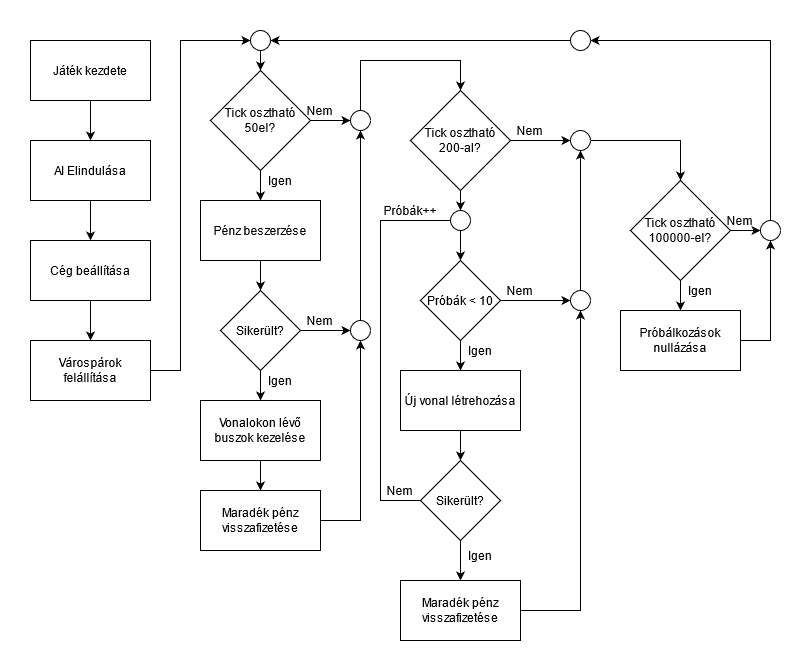
\includegraphics[scale=0.5]{images/folyamat.png}
	\caption{Az AI működésének folyamata}
	\label{fig:folyamat}
\end{figure}

Itt kell kiadnom tehát azokat a parancsokat, hogy új buszvonalak létrejöjjenek a térképen, ehhez lesz majd szükségem a program összes többi elemére, amelyek ezekkel a kisebb problémakörökkel foglalkoznak. Először is fel kell mérnünk a térkép jelenlegi helyzetét, ami alapján az AI meg tudja állapítani az ideális helyet a terjeszkedéshez. Miután ezt a helyet meghatározta, az adott városok között létre kell hoznia az adott buszvonalat, buszmegállókat kell építenie a városokban, össze kell kötnie úttal a városokat, garázst kell építenie az útvonalon, és buszokat kell vásárolnia a vonalra. Azokat a feladatokat amiknek a csoportosítására lehetőség van, mint például a buszmegállók és buszok építése kiemeltem innen és a vonalak kezeléséhez csatoltam, mert logikailag ahhoz a folyamathoz tartozik.

Amit érdemes még itt definiálnunk az a pénzügyek kezelése, mivel ez közvetlenül a céghez tartozik, így logikusabb itt kezelni őket. Szükség lesz egy függvényre ami megszerzi nekünk a terjeszkedéshez a megfelelő anyagi hátteret, valamint egy másikra a munkálatok befejezése után, hogy a korábban kiépített útvonalakból termelt jövedelemből fedezze az esetlegesen felvett kölcsön összegét.

\Section{Városok keresésének módszere}

Ahhoz hogy a játék elején, vagy későbbiekben is, a lehető legtöbb bevételt tudja generálni a program, fontos feladat a megfelelő városok kiválasztása az útvonal megépítéséhez. Ezt a saját stratégia implementációjaként határoztam meg. Egy felhasználó számára ésszerű döntés lehet a legnagyobb népességű városokat összekötni. Ami ténylegesen egy jó megközelítés azonban ez a következő problémákhoz vezethet. A két város túl messze is lehet egymástól ahhoz, hogy az útvonal megbízható legyen. Vagyis a hosszú útvonalon a buszok eltévedhetnek, megfelelő karbantartás nélkül sorozatosan lerobbanhatnak. Ezek miatt pedig romlik az útvonal bevétele és megbízhatósága. Tehát a városok választásánál figyelembe kell vennem azok távolságát is. A túl rövid útvonalakkal is problémákba ütközhet a program, ugyanis, ha túl közel van egymáshoz két megálló, a közte közlekedő buszok hamarabb odaérnek a megállókba, mielőtt a várakozó utasok száma elérné a busz kapacitását, így kihasználatlanul közlekedne az adott jármű.

A városok közötti távolságot méréséhez manhattan távolságot használtam, mivel az elszállítási díj is ezt a távolságot veszi figyelembe. Ilyenkor az API \texttt{AIMap} osztályának \texttt{DistanceManhattan(tile1, tile2)} függvényét segítségül hívva tudtam ezeket az információkat megszerezni. Ahogyan azt az előző bekezdésben megállapítottam, a távolság akkor is hátrányos ha túl alacsony, valamint akkor is, ha túl magas. Ezért feltételezhető, hogy a minimum és maximum érték között található egy olyan távolság, ami az utasok elszállítása szempontjából ideális. Ahhoz, hogy ezt az értéket közelíteni tudjuk, létrehoztam egy algoritmust, aminek a paramétereinek az állításával a későbbiekben kísérleteket tudok tenni, hogy melyik beállítás lenne a legmegfelelőbb. Feltételezzük, hogy a kapott szám a $[0, 1]$ intervallumon helyezkedik el.

\begin{cpp}
function Planner::DistanceMeasure(town1, town2)
{
  local distance = AIMap.DistanceManhattan(AITown.GetLocation(town1),
    AITown.GetLocation(town2)).tofloat();
  local dstar = 50.0;
  local dmin = 30.0;
  local dmax = 100.0;
  if (distance < dmin) {
    return 0.0;
  }
  if (distance < dstar) {
    local result = (distance - dmin) / (dstar - dmin);
    return result;
  }
  if (distance == dstar) {
    return 1.0;
  }
  if (distance <= dmax) {
    local result = 1 - ((distance - dstar) / (dmax - dstar));
    return result;
  }
  if (distance > dmax) {
    return 0.0;
  }
}
\end{cpp}

A számítások elvégzése előtt, segédváltozókban megadom, az algoritmus fixált értékeit, valamint kiszámítom a korábban említett módon a városok távolságát. Ez algoritmus által kiszámított eredmény annál nagyobb lesz, minél közelebb van, az általunk ideálisnak tartott távolságtól.

Másik probléma amibe a fejlesztés alatt ütköztem, hogy a legnagyobb lakosságú város valójában nem az a város, ahol egy megállóval a legtöbb lakost tudja lefedni a program, legyen az egy folyó, vagy túl dombos talaj miatt. A buszmegállók elhelyezéséről és az várható utasok számának becsléséről a későbbiekben részletesen lesz szó. A városok kiválasztásához jelen esetben csak a várható utasok számának becsült értékére van szükség. A térképen található minden város kombinációinak az eleméhez hozzárendeltem az adott városokban a legjobb buszmegállók pozícióinak várható utasszámának összegét. Ezt az értéket normalizáltan a $[0, 1]$ intervallumra azáltal, hogy az adott értéket elosztottam a várospárok közötti maximális értékkel.

Kódrészlet a városok várható utasok számának kiszámításáról és lementéséről:
\begin{cpp}

class Planner {
  town_list = null;
  // Egyéb kód
}

function Planner::BuildTownList()
{
  local manager = TownManager();
  this.town_list = AITownList();
  for (local i = town_list.Begin(); 
   town_list.HasNext(); i = town_list.Next()) {
    local loc = manager.FindStationLocation(i);
    if (loc != false) {
      town_list.SetValue(i, manager.GetStationAcceptance(loc));
    } else {
      town_list.SetValue(i, 0);
    }
  }
  town_list.Sort(AIList.SORT_BY_VALUE, AIList.SORT_DESCENDING);
}
\end{cpp}

Ezt a listát újragenerálja a program, minden alkalommal amikor ideális városokat keres az AI folyamata, ezzel garantálva, hogy a legutóbbi számítások óta történt pályaváltozások miatt ne hibás értékek alapján hozzon döntést. A kódrészletben jól látható, hogy hogyan lehet hasznosítani az API \texttt{List()} osztályát értékek rendezésére. Először minden város elemhez hozzárendelek egy adott értéket, majd egyszerűen a \texttt{Sort()} függvény segítségével sorba lehet rendezni ezeket. Ezekből az adatokból a továbbiakban felépítettem egy háromszögmátrixot, melynek adatai az adott várospárok várható utasszámának értékei. Ennek a kódja itt látható:

Tehát a megfelelő városok kiválasztásánál két fontos tényező a városok távolsága, és az utasok száma amit a városban elhelyezett megálló szolgáltatni tud. Ennek a két változónak a segítségével tudtam felállítani egy egyenletet ami alapján minden várospárt értékelni tud a program a térképen, aztán az egyenlet eredménye szerint eldönteni, hogy melyik az ideális várospár új buszvonal megépítésére. Ehhez az egyenlethez hozzáadtam egy súlyváltozót is, amivel azt tudom befolyásolni, hogy a távolság, vagy az utasok számának hányadosát szeretném inkább figyelembe venni.

Végül az osztály részeként szereplő funkciók az ehhez az egyenlethez szükséges változókat és értékeket állítják elő.

Az így kapott egyenletünk a következő:
\begin{center}
	$ e(i,j)=w_{a} \cdot a(i,j)+(1-w_{a}) \cdot f(d(i,j)) $
\end{center}

Ezt az egyenletet a korábban kiszámított változók segítségével implementáltam, és az eredményt egy tömbben tároltam, a várospár elemeivel és a hozzájuk tartozó $e$ értékkel.

\begin{cpp}
local n = 0;
for (local i = 0; i < townArray.len(); i++) {
  for (local j = i + 1; j < townArray.len(); j++) {
    local d = DistanceMeasure(townArray[i][0], townArray[j][0]);
    local maxacc = GetMaxAcceptance().tofloat();
    local e = (w * ((townArray[i][1] + townArray[j][1]) / maxacc))
      + ((1.0 - w) * d);
    towneArray[n] = [townArray[i][0], townArray[j][0], e];
    n++;
  }
}
\end{cpp}

Itt látható, hogy minden várospárra elvégződik a számítás, meghívódik a bemutatott távolságfüggvény, ami az egyenletben $f(d(i,j))$ képpen szerepelt. A \texttt{GetMaxAcceptance()} függvény egy egy segédváltozót határoz meg amire a várható utasok számának normalizálása miatt van szükség, ez az érték a maximuma lesz a várospárok között lévő várható utasoknak. Az eredményül kapott \texttt{towneArray} minden eleme tehát egy várospár, és a hozzá tartozó $e$ érték. Ennek a tömbnek az egyszerű buborékrendezése után, kaptam egy rendezett listát a terjeszkedésre ideális városokról.

Az egyenlet paramétereinek változtatásáról, és annak az eredményeiről a tesztelés fejezetben lesz részletesebben szó.

\Section{Városkezelő}

A városkezelő osztálynak a részét képezik azok a függvények amik az infrastruktúra építés szempontjából kihatnak a városokra, vagy azokról szolgálnak információval.

Az egyik ilyen függvény amely meghatározza hogy egy városon belül melyik mező lenne a legalkalmasabb egy megálló építésére, ez a programban a \\ \texttt{FindStationLocation(townid)}, ami bemeneti értékként a vizsgálandó várost várja. Ennek a pozíciónak a kiválasztása egy fontos feladat a cég bevételének növeléséhez, mivel minél több házat tud a program lefedni egy megállóval, annál több utast képes elszállítani onnan. A megállóknak két típusa van, az egyik az útra építhető, két végén rendelkezik ki és bejárattal, valamint egy pályaudvar szerű, aminek csak az egyik oldalon van bejárata. Az algoritmus fő célja megtalálni azt a pozíciót a városban ahol a lerakott állomás lefedettségében a várható utasok száma a legnagyobb. A különböző állomások típusait \aref{fig:megallok} ábrán láthatjuk. Ezt egy olyan városban ahol még egyáltalán nem található meg állomás viszonylag könnyű meghatározni, mert nem kell a cégek közötti vagy a saját megállók közötti versengéssel számolni.

\begin{figure}
	\centering
	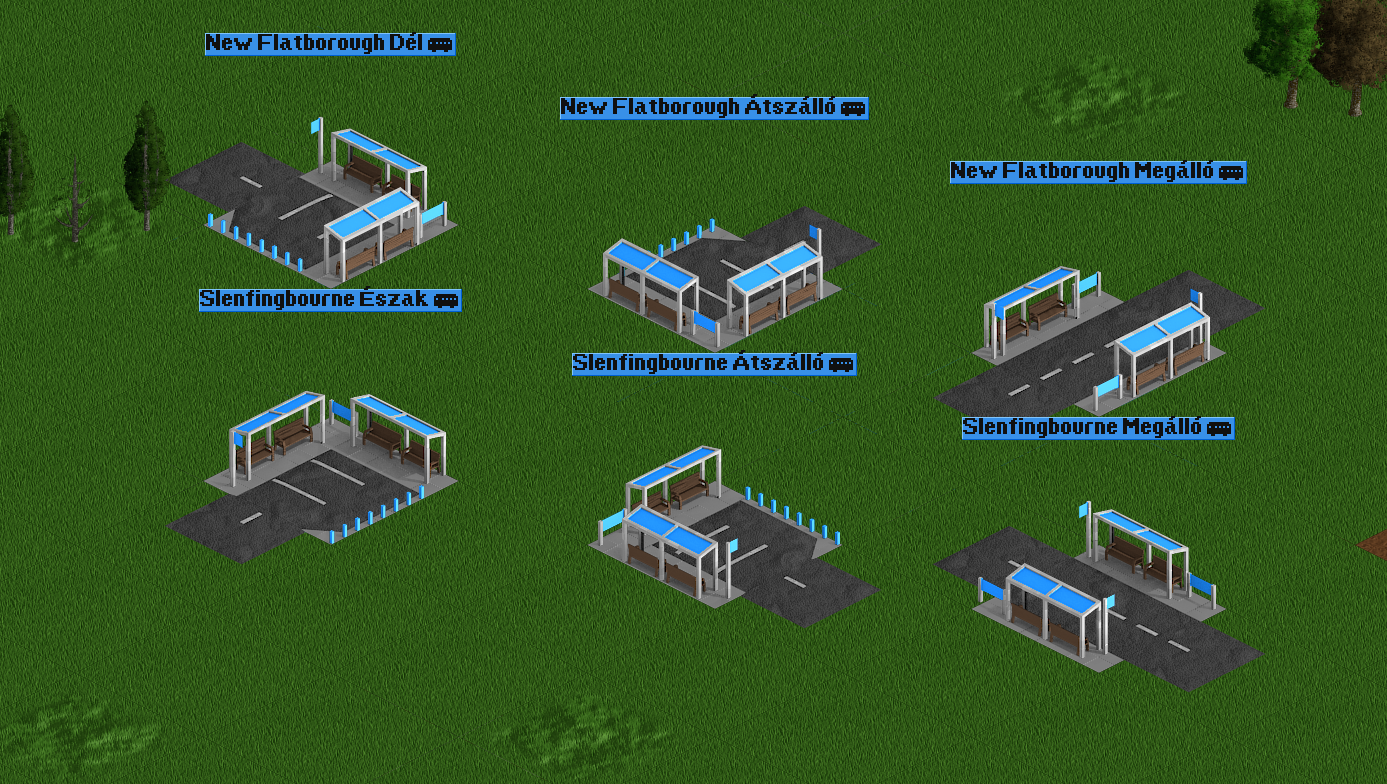
\includegraphics[scale=0.4]{images/megallok.png}
	\caption{Buszmegállók típusai}
	\label{fig:megallok}
\end{figure}

Ahhoz hogy meghatározzam melyik mező lenne a legalkalmasabb, először szükségem volt egy listára amely tartalmazza a város körüli mezőket, majd ezek tulajdonságai alapján tud a program döntésre jutni. Az API-nál említett \texttt{AITileList} egy hasznos osztály ebben az esetben, ugyanis az \texttt{AddRectangle()} függvényével hozzá tudtam adni a város környezetében található mezőket, majd azokat a \texttt{Valuate()} segítségével hozzá tudtam rendelni értékeket különböző feltételek alapján, és az értéktől függve megtartani vagy eldobni az elemeit. Elsősorban kizártam a hiba lehetőségét azzal, hogy ellenőriztem a listában található elemek mind érvényes mezők-e, másodkörben pedig elvetettem minden olyan mezőt ami víz mezőnek számít, legyen az folyó, tó vagy a pálya szélén található tenger egy mezeje.

\begin{cpp}
function TownManager::FindStationLocation(town_id) {
  local tl = AITileList();
  
  tl.AddRectangle(town_loc + AIMap.GetTileIndex(-8, -8),
   town_loc + AIMap.GetTileIndex(8, 8));
   
  tl.Valuate(AIMap.IsValidTile);
  tl.KeepValue(1);
  tl.Valuate(AITile.IsWaterTile);
  tl.KeepValue(0);
  
  if (tl.Count()) {
    tl.Valuate(AIRoad.GetNeighbourRoadCount);
  	tl.KeepAboveValue(0);
  	if (tl.Count()) {
      tl.Valuate(AITile.GetSlope);
      tl.KeepValue(0);
      if (tl.Count()) {
      	// Maradék mezők vizsgálata a várható utasszámra
      }
    }
  }
}
\end{cpp}

Amennyiben a listában még vannak elemek, a program folytatja a szűrést olyan mezőkre, amelyek legalább egy másik olyan mezővel szomszédosak, amin út található és aztán olyanokra, amelyek nem lejtenek. Ezekre a szűrésekre két dolog miatt van szükség. Az első, hogy elkerüljük az olyan szituációkat, hogy egy $3 \times 3$-as terület közepén aminek a szélein épületek vannak, találjunk ideális megállót, azonban ahhoz hogy a megállót összekössük úttal, le kell rombolnunk az egyik épületet, ezzel rontva a szolgáltatott utasok számát a megállóban. A lejtőket pedig az állomások sajátosságba miatt kell kiszűrni. Ugyan az utak, a kanyarok kivételével épülhetnek lejtőkre, az útra építhető állomások nem, valamint van esély arra is, hogy olyan út melletti mezőt találjon a program, ami egy lejtő, és a ráépített állomás a lejtő tetején foglalna helyet. Azonban ha a szomszédos út amihez csatlakoztatnunk kellene egy lejtő, vagy mélyebben helyezkedik el nem tudjuk összekötni a megállót az úthálózattal. Ezt a problémát szemlélteti \aref{fig:lejtomegallo} ábra. Ha az adott mezőn út található, elvégez egy vizsgálatot a program ami meghatározza, hogy tud-e olyan megállót építeni rá, amin keresztül lehet haladni. Ezt az alapján teszi meg, hogy megvizsgálja a környező mezőket, és hogy azok utak-e, és csak azt a lehetőséget hagyja fent, amikor csak az állomás két végén található mező út, ugyanis kanyarra, vagy T vagy X kereszteződésre nincs lehetőség ilyen típusú állomás építésére.

\begin{figure} [h!]
	\centering
	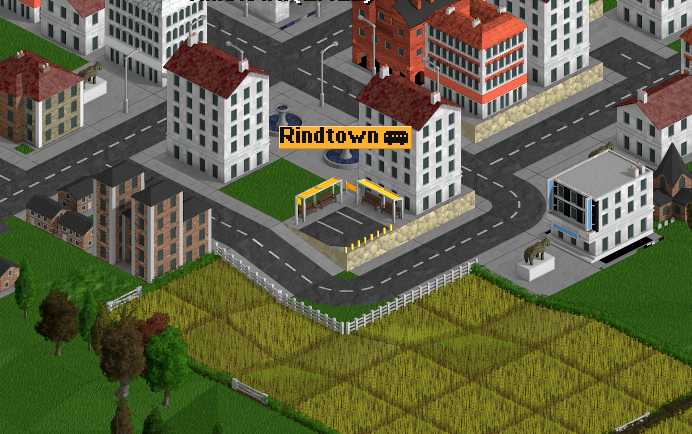
\includegraphics[scale=0.8]{images/lejtomegallo.png}
	\caption{Buszmegálló út mellett, de lejtőn, a megálló nem csatlakozik az úthálózathoz.}
	\label{fig:lejtomegallo}
\end{figure}

A szűrések elvégzése után már csak olyan mezők maradtak amire a program tud megállót építeni, már csak az maradt hátra hogy meghatározza, hogy ezek közül melyikre lenne a legérdemesebb. Ennek az elősegítésére létezik az API-ban az \\ \texttt{AITile.GetCargoAcceptance()} függvény, amelynek paraméterként átadom a mezőt amelyen az állomást építeni szeretném, az árú típusát, ami jelen esetben az utasok, valamint a megálló dimenziót, és a sugarat, amekkora területet lefed a buszmegálló. Ezzel a függvénnyel azonban egy problémába ütköztem, amit az API nem is közöl velünk. Ez a függvény mindig a maximális értéket adja vissza a lefedett területről, azaz, nem veszi figyelembe a más cégek, vagy a saját buszmegállóink lefedettségének ütközését, ahol a többszörösen lefedett területekről szolgáltatott utasok arányosan oszlanak el a megállók között.

Ezért volt szükséges egy saját függvény létrehozása, ami pontosabban tudja megbecsülni az buszmegálló által lefedett utasok számát. Így lett létrehozva a \\ \texttt{GetStationAcceptance(tile)}, amely bemeneti értékként azt a mezőt várja, ahova a buszmegállót építeni szeretnénk.

Ez a függvény először lekérdezi az adott mező körülötti területet amit szükséges megvizsgálnia annak érdekében hogy van e átfedés a megállók között. Mivel a buszmegállók csak egy mezőt foglalnak el, és $7 \times 7$-es területet fednek le, ahol a terület közepén helyezkedik el az állomás. Így az a terület amit vizsgálnunk kell az a megálló körül vett, legalább 6 sugarú terület, ugyanis, ha még az állomástól számított 6. mezőn van egy állomás, akkor legalább egy oszlopban átfedés lesz. Azonban ha már a 7. van azt nem érdemes azt megvizsgálni, mivel pont szomszédos mezőket fednek csak le. A buszmegállók által lefedett területről \aref{fig:megallo} ábrán láthatunk példát, itt a rivális cég megállója 5 távolságra van, a két megalló lefedettsége 2 oszlopban is fedi egymást. Abban az esetben, ha a program nem talál másik állomást a vizsgált területen belül, egyszerű dolga van, mivel tudjuk használni az API által szolgáltatott függvényt. Amennyiben talált állomást, a megoldás kicsit bonyolultabb lesz. Először is létrehoztam egy listát amiben eltároltam az általunk lerakandó megálló által lefedett mezőket és minden mező értékét 1-re állítottam, aztán egy segédlistában pedig eltároltam azokat a mezőket, amelyek egy adott már meglévő megálló által le vannak fedve. Végigiterálva az általam lerakandó állomás által lefedett mezőkön, a program összehasonlítja, hogy az adott mező szerepel-e a segédlistában. Amennyiben igen, a \texttt{List()} értékmezőjében lévő értéket növelem egyel. Ha végigiterált a program az összes elemen és összes megállón, akkor a lista segítségével ki tudja számítani a valódi utasok számát. Lekérdezem a \texttt{GetCargoAcceptance()} segítségével minden egyes mezőre jutó utasszámot amit elosztok az adott elem értékével, ami 1, ha nem volt átfedés más állomással, így az adott érték az alapértelmezett marad, azonban ha volt átfedés, a kapott eredmény annyiad részét kapom eredményól, ahány megállóval van átfedésben a mező. Végül pedig visszaadom a kapott értékek összegét.

\begin{figure} [b!]
	\centering
	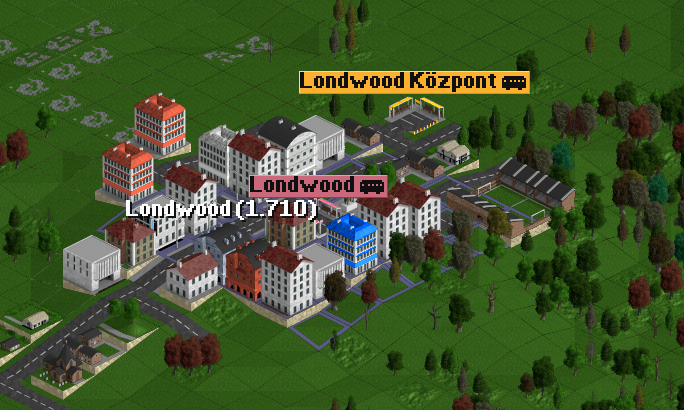
\includegraphics[scale=0.8]{images/megallo.png}
	\caption{Buszmegálló által lefedett terület (lila körvonal)}
	\label{fig:megallo}
\end{figure}

Ha a \texttt{FindStationLocation()}-ben megkapott mezőkre meghívom a \\ \texttt{GetStationAcceptance()} függvényemet, és a kapott értékeket lementem a lista részeként, egy egyszerű \texttt{Sort()} segítségével csökkenő sorrendbe is tudom rendezni, és az így kapott lista első eleme lesz a legtöbb várható utassal rendelkező állomás pozíciója.

\begin{cpp}
if (!AITile.IsBuildable(tile)) {
  AILog.Info("Demolishing tile: " + tile);
  demolished = AITile.DemolishTile(tile);
} else {
  demolished = true;
}
if (demolished) {
  for(local tile2 = adjacentTiles.Begin(); 
   adjacentTiles.HasNext() && !built; tile2 = adjacentTiles.Next()) {
	if (AIRoad.IsRoadTile(tile2)) {
      builder.RoadBuilder(tile2, tile);
      built = AIRoad.BuildRoadStation(tile, tile2,
      AIRoad.ROADVEHTYPE_BUS, AIStation.STATION_NEW);
      builder.RoadBuilder(tile2, AITown.GetLocation(town_id));
    }
  }
}
\end{cpp}

A városkezelő utolsó függvénye a buszmegálló építő \texttt{BuildStation(tile, townid)}. Ennek meghíváskor átadom a mezőt ahova az állomást szeretném építeni, valamint a várost ahova építeni szeretném. Az utóbbira azért lesz szükségem, hogyha menetközbe megszakadt volna az útvonal a megálló és a város között, akkor össze tudja a függvény kötni őket úttal. Itt már csak azt kell meghatároznom, hogy az adott mező amire építeni szeretném a megállót út-e vagy sem, és a mezőre tudok-e építkezni vagy sem. Az első vizsgálatra a megálló típusának kiválasztása miatt van szükség, ha az adott mező út el kell dönteni, hogy az építendő megálló fentről lefelé, vagy balról jobbra vezető megálló lesz. Ha a mező nem út, akkor azt kell eldönteni, hogy a szomszédos mezők közül melyik az, hogy hozzá tudjam kötni a megállónkat az úthálózathoz. Az utóbbira pedig akkor, ha a mező nem egy út, de a mezőn valami megakadályozza hogy állomást építsek oda. Abban az esetben, ha valami akadályozza az építkezést, a mezőt lerombolom és úgy próbálkozok megépíteni a megállót. Ha a megálló sikeresen megépült, akkor a biztonság kedvéért összekötöm a megálló előtti mezőt a város központjával. Amennyiben a két mező között már volt úthálózat, nem történik építkezés.

\Section{Építkező}

Ez az osztály tartalmazza az útvonalkereső függvényt, ami valójában a keretrendszer részeként szolgáltatott \texttt{RoadPathfinder} egy implementációja. Valamint megtalálható még egy segédfüggvény, amivel egy adott mező szomszédos mezőit tudom lekérdezni, ami sok építkezésnél hasznos információkkal tud szolgálni.

Az útvonalkeresőről a játék weboldalán találhatunk részletes leírást, valamint segédletet az implementációhoz. Valójában az AI-ban található implementáció is a weboldalon megtalálható egy minimális átformálása. Ennek a függvénynek csak két mező típusú objektumot kell megadnom, ami alapján az algoritmus a megadott paraméterek alapján összeköti ezeket és visszaadja az útvonalat egy path objektum formájában. Ha ezt az útvonalat megkaptam, már csak az útvonal mezőire kell utat építenem, és van is egy működő algoritmusom két pont összekötésére.

Az útvonalkereső használatához importálnunk kell a programba a \\ \texttt{pathfinder.road}-ot. Ez által érhető el az útvonalkereső funkciói. Az ebben lévő osztálynak kell egy példányát létrehoznunk, aminek a segítségével már kereshetjük is az útvonalak apróbb beállítások után.

\begin{cpp}
import("pathfinder.road", "RoadPathFinder", 3);

function Builder::RoadBuilder(start, goal) {
  AIRoad.SetCurrentRoadType(AIRoad.ROADTYPE_ROAD);
  local pathfinder = RoadPathFinder();
  pathfinder.InitializePath([start], [goal]);
  
  local path = false;
  while (path == false) {
    path = pathfinder.FindPath(100);
    AIController.Sleep(1);
  }
}
\end{cpp}

Az adott kódrészlet, a függvény paramétereiben átadott start és goal mezők között meg is kezdi az útvonal keresését. Ha sikeresen talált útvonalat, azt egy path objektumkban el is menti. Ha még folyamatban van az útvonal keresése, \texttt{false} értéked ad vissza, ha pedig nem talált útvonalat \texttt{null}-t. A függvényhívásnál szereplő 100-as érték az iterációk számát jelöli.

Az útvonalkereső algoritmus valójában egy A* algoritmus alapvető implementációja. Ez határozza meg a paraméterek szerinti "legolcsóbb" útvonalat. Példa az átállítható paraméterekre például a kanyarok költsége, alagutak vagy hidak használatának költsége, lejtők használatának költsége.

\Section{Útvonalkezelő}

Az útvonalak kezeléséhez szükségem van egy osztályra, amelynek a példányaiban lehetőség van eltárolni az összes adott vonalhoz tartozó információt. Ennek az osztálynak a felépítése látható \aref{fig:line} ábrán. A programban ez az osztály felelős az egyes útvonalak felállításáért, ide értve a hozzá tartozó infrastruktúra felépítését és a elemeinek kezelését is. Az útvonal felépítéséhez szükséges feladatokat ellátó függvényekről már korábban esett szó. Itt a \texttt{CreateNewLine(townpair)} függvény foglalja össze ezeket.

\begin{figure}
	\centering
	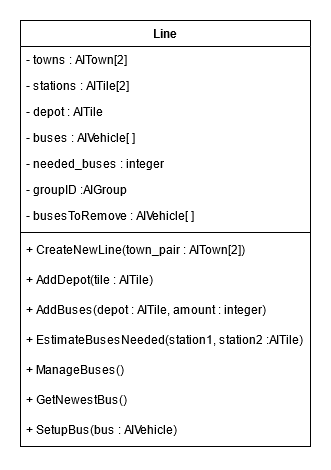
\includegraphics[scale=0.5]{images/line.png}
	\caption{A \texttt{Line} osztály felépítése.}
	\label{fig:line}
\end{figure}

Ennek a függvénynek kell megkapnia az összekötendő városokat, ami alapján meghívja a többi szükséges osztályt a buszmegállók helyeinek meghatározására és megépítésére. Itt kell lekezelni azt a problémát is, ha valamelyik városban nem sikerülni különböző okok miatt a buszmegálló megépítése. Mivel nem is tudjuk egyszerre megépíteni, az is előfordulhat, hogy az egyik megálló már megépült, mire a másikról kiderül, hogy nem tudja megépíteni az AI. Ezért oda kell figyelni, hogyha az első megálló megépült, de a második nem, akkor az első megépített megállót eltávolítsa. Ha nem sikerült már az első megálló építése sem, azonnal megszakítjuk a folyamatot. Amennyiben minden építkezés sikeresen lezajlott az osztály többi függvénye megépíti és lementi az útvonalhoz kapcsolt garázst majd megvásárolja a szükséges mennyiségű járművet. Ezután pedig kiadja a megfelelő utasításokat a buszoknak, hogy melyik megállóba kell eljutniuk, aztán elindítja őket. Ez a folyamat megvalósítása több kisebb problémához vezetett amikkel külön kellett foglalkoznom.

Kódrészlet a buszmegállók építésének vizsgálatáról.
\begin{cpp}
if (stops[0] && stops[1]) {
  builtstation.append(manager.BuildStation(stops[0], town_pair[0]));
  if (builtstation.top() != false) {
    stations.append(stops[0]);
    builtstation.append(manager.BuildStation(stops[1], town_pair[1]));
    if (builtstation.top() == false) {
      AILog.Info("Failed to build second station");
      stations.pop();
      AIRoad.RemoveRoadStation(stops[0]);
      return false;
    }
    stations.append(stops[1]);
  } else {
    AILog.Info("Failed to build first station");
    return false;
  }
} 
\end{cpp}

Ahhoz hogy buszokat tudjon vásárolni a cég először is egy garázsra van szüksége, ahol ezeket a buszokat el tudja tárolni és a későbbiekben karbantartani, vagy elöregedésük után eladni. Ennek a garázsnak a pozíciójának a meghatározása hasonló folyamat az megállók helyének meghatározásával, leszámítva a lefedett területek bonyolultságát. Erre készítettem egy függvényt \texttt{AddDepot(tile)} néven, aminek megadom a városhoz tartozó megálló pozícióját. Aztán vettem a megálló körüli területet egy sugárral, és megvizsgálom hogy a városban építettem-e már korábban garázst, ugyanis ha igen ezt érdemes újrahasználni, mivel a megállókkal ellentétben ennek nincs negatív hatása az utasokra, azonban megspórolhatom vele egy felesleges garázs fenntartási költségeit.

Abban az esetben ha még nincs garázs a körzetben, veszek minden olyan mezőt egy körzetben ami nem lejt, út mellett helyezkedik el és önmaga nem út. A megmaradt mezők közül kiválasztom azt, amelyik a legközelebb van a vonalhoz tartozó másik városhoz. Erre nem feltétlen lenne szükség, de így nagyobb valószínűséggel helyezzük el a garázst olyan pozícióban, ami olyan úttal szomszédos amin a két megálló között közlekedve elhaladnak a járművek. Ha a függvény talált alkalmas mezőt a garázsnak, megvizsgálja tud-e építkezni a mezőre, és ha igen elhelyezi a garázst.

\begin{cpp}
searchedArea.AddRectangle(tile + AIMap.GetTileIndex(-15, -15),
 tile + AIMap.GetTileIndex(15, 15));

searchedArea.Valuate(AIRoad.IsRoadDepotTile);
searchedArea.KeepValue(1);

if(!searchedArea.IsEmpty()) {
  for (local i = searchedArea.Begin(); 
   searchedArea.HasNext(); i = searchedArea.Next()) {
    if (depos.HasItem(i)) {
      AILog.Info("Existing depot found");
      return i;
    }
  }
}
\end{cpp}

A garázs meglétével már lehetőség van új járművek vásárlására. Mielőtt költekezésbe kezdene a cég, érdemes kiszámítani egy közelítő értéket, hogy hány buszra lesz szüksége, hogy a várható utasmennyiséget le tudja fedni a vonalon. Ebből a célból létrehoztam egy \texttt{EstimateBusesNeeded(station1, station2)} függvényt. Ez egy egyszerű egyenlet segítségével készít egy becslést a szükséges buszok számáról. Az alap érték legalább 2, mivel szeretném, hogy mindkét megállóban legyen egyszerre legalább egy busz és ezek forogjanak a megállók között. A számításnál figyelembe veszem még a vonal állomásai által lefedett várható utasok számát, az állomások egymástól vett távolságát és a buszok férőhelyeit. A visszaadott érték a becsülten szükséges buszok száma. Ezt az értéket pontosan nem fogom tudni megállapítani, mivel a véletlenszerű tényezők amik befolyásolják a buszok haladási sebességét, például a lerobbanás, vagy kereszteződésben való várakozás is befolyásolhatja a buszok menetidejét.

\begin{cpp}
function Line::EstimateBusesNeeded(station1, station2)
{
  local manager = TownManager();
  local acceptance = manager.GetStationAcceptance(station1) +
   manager.GetStationAcceptance(station2);
  local distance = AIMap.DistanceManhattan(station1, station2);
  local estimatedBuses = 2 + (acceptance/35) * (distance/35);
  if (estimatedBuses > 25) {
    estimatedBuses = 25;
  }
  return estimatedBuses;
}
\end{cpp}

Már az algoritmus által becsült buszok számának birtokában, szükségem van egy folyamatra, ami ezeknek a buszoknak a megvásárlását elvégzi. Erre a célra alkottam meg az \texttt{AddBuses(depot, amount)} függvény. A depot-tal adom meg hogy melyik garázsba szeretném építeni az adott buszokat, az amount-tal pedig vásárolandó buszok számát, ami alap esetben a becsült buszok száma.

Először is meg kellett határoznom, hogy milyen típusú járművet szeretnék vásárolni. Erre azért van szükség, mivel a játékbeli idő előrehaladtával újabb járművekhez van hozzáférése a cégeknek, amik modernebbek, nagyobb férőhellyel rendelkeznek vagy megbízhatóbb működésűek. Az egyszerűség kedvéért, én csak a legnagyobb férőhelyű busszal foglalkoztam az adott buszok listája közül. Ennek a busztípusnak a meghatározását egy külön függvénybe rendeztem, mivel a buszok karbantartásánál is hasznos lesz a legnagyobb kapacitású busz meghatározása.

Ha sikeresen döntésre jutott az AI a busz modellről, már csak meg kell vásárolnia az adott számú darabot belőle. Esetleg ha ez a folyamat nem lenne sikeres egyéb okok miatt, például a cégnek nincs elég pénze 10 buszra csak 7-re, abban az esetben a maradék 3-at amit nem sikerült megvásárolni, eltároltam a vonal változói között, hogy később, amikor a cég rendelkezik elegendő pénzmennyiséggel, újra megpróbálja megvásárolni ezt a 3 járművet.

Miután rendelkezem minden elemmel ami a vonal működéséhez szükséges, ide értve a buszmegállókat, az úthálózatot a városok között, a garázst és a buszokat, az utolsó feladat a parancsok kiosztása a buszoknak, és az elindításuk. Ezt a feladatot a \texttt{SetupBus(bus)} függvény látja el, ami hozzáadja egy csoporthoz a járművet, amely vonalanként különböző aztán a vonal változói között található buszmegállókba, és a vonalhoz tartozó garázs-t kiadja parancsként. A parancsoknak több típusa van, ha nem határozunk meg kifejezetten egyet, az alapértelmezett parancs a "lerakodás ha van mit, és felrakodás ha van mit" az állomások esetén. Egy garázs parancs esetén ez "karbantartás a garázsban, ha szükséges" parancsot jelenti. Ennek a függvénynek a lefutása után a vonal életbe lép és aktívan látogatja a hozzá tartozó megállókat a buszaival. \Aref{fig:vonal} ábrán látható egy aktív útvonal használatban.

\begin{figure}
	\centering
	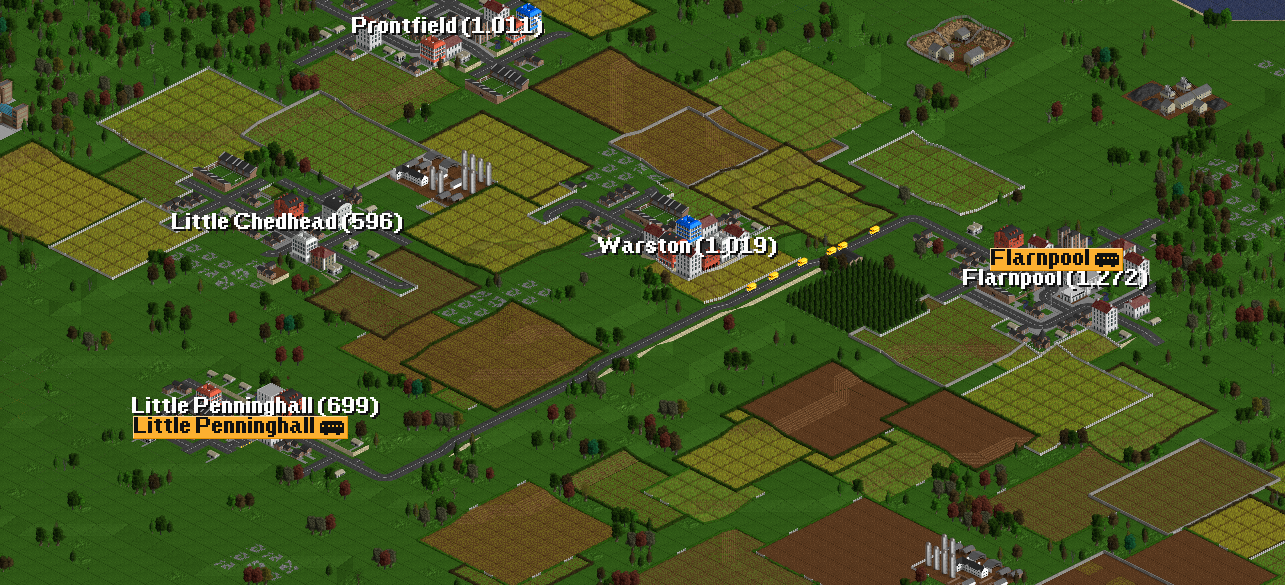
\includegraphics[scale=0.45]{images/vonal.png}
	\caption{Egy aktív vonal buszmegállókkal, garázzsal és buszokkal.}
	\label{fig:vonal}
\end{figure}

Az utolsó ide tartozó függvény a \texttt{ManageBuses()}. Erre a függvényre azért van szükség, hogy a buszokat amelyeket nem sikerül az első folyamatban megvásárolni, később újra tudja próbálni a program. Valamint a folyamat időközönként újra ellenőrzi a szükséges buszok számát és összehasonlítja a jelenleg futó buszok számával.Végső soron pedig kezeli az elöregedő buszok lecserélésének folyamatát.

A hiányzó buszok pótlása egy egyszerű feladat, csak ellenőriznie kell a programnak, hogy van e szükség újabb buszok vásárlására és ha igen, a korábban bemutatott függvény segítségével pótolni tudja a ezeket. Amennyiben ismételten nem lenne elég pénze a cégnek a buszokra, az értéket megfelelően változtatja a továbbra is hiányzó buszok számára.

Ha a korábbi becsléssel megegyező számú busz fut a vonalon, akkor újra ellenőrzi a szükséges buszok számát. Erre azért van szükség, mert egy rivális cég vagy saját cégünk újonnan épült megállója átfedésbe kerülhet a korábban szabad megállóval, emiatt a várható utasok száma is változhat. Vagy egy másik ok a változásra a városok növekedése. Előfordulhat hogy egy vonal éveken keresztül használatban van egy városban, aminek hatására a város növekedni kezd, több ház épül a területen, vagy korábbi kis lakóházak a város központjában nagyobb irodaházakra épülnek át. Ezért érdemes figyelmet fordítani ezekre a folyamatokra is. Így ha az újrabecsült érték magasabb mint a jelenleg futó buszok száma, növelem a szükséges buszok értékét és megpróbálom megvásárolni azokat. Abban az esetben, ha az újrabecsült érték alacsonyabb mint a buszok száma a vonalon, akkor a különbségükkel egyenlő számú buszt eltávolítok a vonalról.

\begin{cpp}
if (this.needed_buses != 0) {
  // Hiányzó buszok megvásárlása
} else {
  local newEstimate = 
    EstimateBusesNeeded(this.stations[0], this.stations[1]);
  if (this.buses.len() < newEstimate) {
    AILog.Info("Adding additional buses to line");
    this.needed_buses = 
      AddBuses(this.depot, (newEstimate - this.buses.len()));
    for (local i = 0; i < this.buses.len(); i++) {
      if (AIVehicle.IsStoppedInDepot(this.buses[i])) {
        SetupBus(this.buses[i]);
      }
    }
  } else if (this.buses.len() > newEstimate) {
      AILog.Info("Removing Vehicles from line");
      for (local i = 0; i < (this.buses.len() - newEstimate); i++) {
        local removedBus = this.buses.pop();
        AIVehicle.SendVehicleToDepot(removedBus);
        this.busesToRemove.AddItem(removedBus, 0);
  }
}
\end{cpp}

Az elöregedő buszok lecserélése közben is el kell távolítanom adott buszokat a vonalról, mielőtt ezt megteszem, megvizsgálom, hogy a jelenleg legnagyobb férőhelyű busz ugyan az a modell-e mint az elöregedett busz. Amennyiben igen, az öreg buszt klónozom. A klónozás folyamata közben a cég vesz egy ugyan olyan modellű buszt a vonal garázsába, ami már alapértelmezetten rendelkezik a korábbi busz parancsaival. Ha más modellt kapunk, abban az esetben megvásárolom az új buszt, hozzáadom a buszok listájához és kiadatom neki a vonalhoz tartozó parancsokat majd elindítom, miközben megkezdem a régi busz eladását.

\begin{figure}[h!]
	\centering
	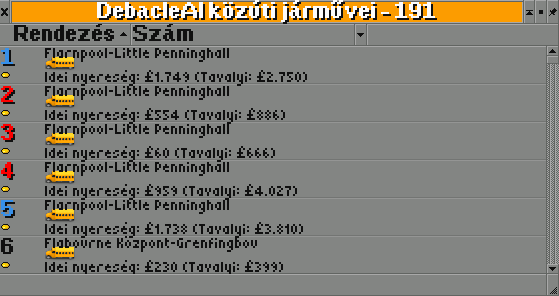
\includegraphics[scale=1]{images/buszok.png}
	\caption{Cég buszainak listája, Elöregedett buszok (piros), Garázsban várakozó buszok (Kék) és aktív buszok (fekete)}
	\label{fig:vonal}
\end{figure}

Az buszok eltávolítása közben egy olyan problémába ütköztem, hogy csak olyan buszok eladására van lehetőségünk, amelyek egy garázsban vannak leállítva. Tehát, amikor el akarok adni egy járművet, először ki kell adnom a parancsot hogy menjen a legközelebbi garázsba, aztán ha látom, hogy az adott busz megállt tudjuk csak eladni. Egy busz esetében ez nem is lenne nagy hatással a programra, viszont mivel a vonal felépítésekor egyszerre több buszt is vásárolunk, ezek egyszerre fognak kiöregedni is. Így ha minden buszra egyesével kellene várnia a programnak míg befut a garázsba és eladásra kerül, jelentős futási időt pazarolna el az AI, amit akár új vonalak létrehozására is szánhatna. Ezért minden elöregedett vagy eladásra váró buszt először eltávolítok a buszok listájából, és hozzáadom az eladásra váró buszok listájához. Ezt a listát a járművek kezelése előtt ellenőrzöm, hogy az ebben szereplő buszok beérkeztek-e már a garázsba és amennyiben igen, eladom azokat. Így párhuzamosítva az eladás folyamatát a program többi részével.
